\section{Q16: reconstructing hidden structure does not improve the decision signal}
\label{sec:q16}

\textbf{Reconstructing the hidden book more accurately did not make the final prediction
better.} This is the paper's cleanest result and its most counterintuitive one. A coarse
limit-order-book view discards the individual resting orders behind an aggregate volume,
and a natural pipeline tries to recover them: estimate the hidden queue sizes and
near-touch depth, feed those estimates to the predictor, and expect a lift. We built that
pipeline on real BTC breakout and rebound cohorts and measured the lift directly.

\paragraph{Setup recap.} On seven monthly cohorts (May through November 2025) we compare
the coarse predictor C, the reconstruction-augmented predictor P, and the observed-rich
predictor R under the identical model, budget, and dates of Section~\ref{sec:setup},
scoring the multiclass target with half-Brier loss. Reconstruction quality is measured
separately: every hidden summary that P consumes is compared to a frozen target-mean
baseline, and on every cohort each summary is recovered \emph{more} accurately than that
baseline. The question is whether that recovered accuracy survives to the decision.

\paragraph{It does not.} Figure~\ref{fig:reconstruction} reads the August cohort, the
largest at $691$ events. The augmented predictor P scores a half-Brier loss of $0.35692$
against the coarse predictor's $0.35286$: augmenting with reconstructed structure made the
prediction \emph{worse} by $0.00405$. It is also $0.01762$ worse than the
training-frequency baseline, a predictor that ignores the current book entirely and
replays the training class mix. The observed-rich predictor R does not rescue the story:
it is $0.01793$ worse than C on the same cohort. Better recovered inputs, and even the
true rich inputs, bought a worse decision signal.

\begin{figure}[t]
\centering
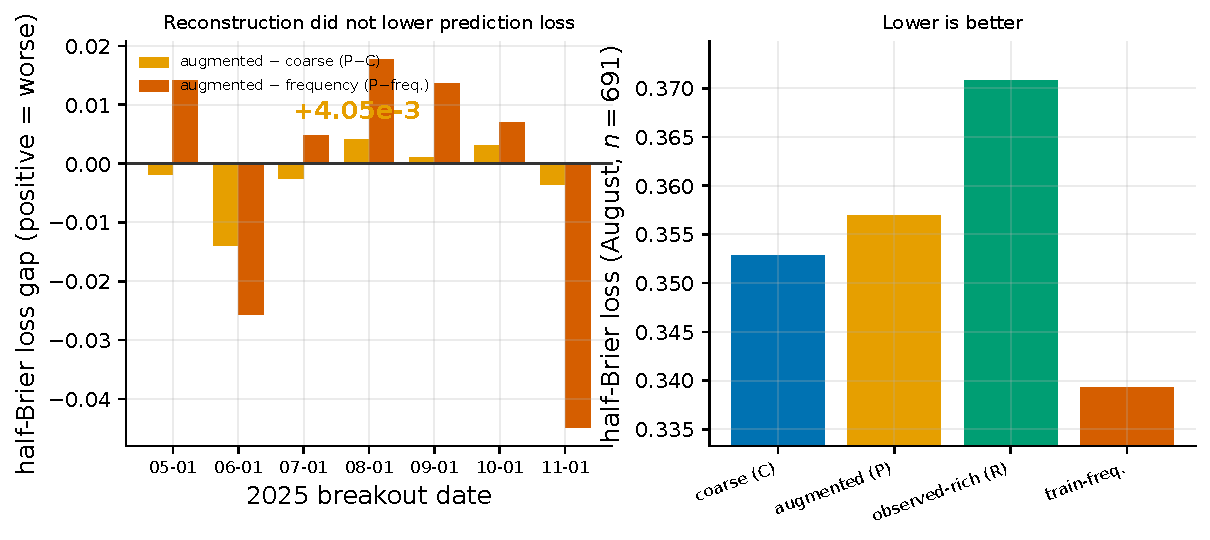
\includegraphics[width=\linewidth]{figures/fig_reconstruction.pdf}
\caption{\textbf{Q16: more accurate reconstruction, no better prediction.}
\textbf{Left:} per-date half-Brier loss gap of the augmented predictor P against the
coarse predictor C (positive means P is worse) and against the training-frequency
baseline. P is worse than the frequency baseline on the majority of dates. The August
cohort ($n=691$) is annotated at $+0.00405$.
\textbf{Right:} absolute August losses for coarse (C), augmented (P), observed-rich (R),
and training-frequency. Lower is better. Neither reconstruction nor the true rich view
beats coarse, and none beats the book-free frequency baseline.}
\label{fig:reconstruction}
\end{figure}

\paragraph{The pattern is not a single unlucky day.} Pooling the four August--November
breakout dates under equal-day weighting ($n=1749$), P remains above C ($+0.00118$
half-Brier) and R remains above C ($+0.00318$). No learned breakout arm beats the
training-frequency reference under event weighting, and on the earlier development dates
the learned arms lose to frequency as well. An earlier aggregate that had appeared to
favor rich depth disappeared once models were frozen and re-scored on held-out months:
the apparent gain was a class-mix and aggregation artifact, localized by a post-hoc
decomposition that separates the class-mixture term from the within-class term.

\paragraph{Controlled mechanism.} To check that this is not an estimation failure specific
to the market pipeline, we reproduce it in a controlled synthetic setting where the hidden
state and the optimal decision are known. There, restricted summaries incur $0.075$
decision regret, but a matched direct predictor and the posterior-restoration predictor
produce \emph{equal} decision coordinates: hidden-queue uncertainty matters, yet
reconstruction carries no isolated advantage over predicting the decision directly, and at
$512$ training draws the direct and distributional outputs coincide. A conditional shift
that is invisible in the observation marginal harms both approaches identically. The
mechanism is general: reconstruction spends capacity recovering structure that the
decision does not need.

\paragraph{The finite-queue special case.} The original Q16 question, can knowing the
\emph{count} and identity of individual orders narrow which fills are feasible?, has a
clean constructed answer that points the same way. In a finite FIFO model over $1000$
histories, aggregate volume alone leaves $59$ histories ambiguous, and adding displayed
order counts leaves $19$. Counts narrow the feasible outcome in $40$ of $1000$ histories.
The information is real but rare. On admitted native Hyperliquid observations the same
count-tightening was not established ($0$ of $961$ in the conditional cohort), and the
mandatory native-FIFO endpoint requires an order-lifecycle archive we located but have not
yet fully processed (Section~\ref{sec:synthesis}). The decision-relevance evidence for Q16
therefore rests on the reconstruction diagnostic above, where the answer is unambiguous:
recovering hidden structure did not help the decision.
